%!TEX root = ../../TD/TD_template_CoursIsenLaTeX.tex
\documentclass[../../TD/TD_template_CoursIsenLaTeX.tex]{subfiles}

\begin{document}

\begin{Exercice}
 \label{ex:CH2:ex1} Attracteur de Lorenz
\end{Exercice}

L’attracteur de Lorenz est une structure fractale correspondant au comportement à long terme de l'oscillateur de Lorenz. L'attracteur montre comment les différentes variables du système dynamique évoluent dans le temps en une trajectoire non périodique. Ce système dynamique s'écrit :
\begin{empheq}[left = \empheqlbrace]{align*}
 \dot{x_1} &= -\sigma x_1 + \sigma x_2\\
 \dot{x_2} &= \rho x_1 - x_2 - x_1x_3\\
 \dot{x_3} &= x_1x_2 - \beta x_3
\end{empheq}
avec $\sigma, \rho, \beta$ trois entiers strictement positifs.

\begin{figure}[!ht]
 \center
 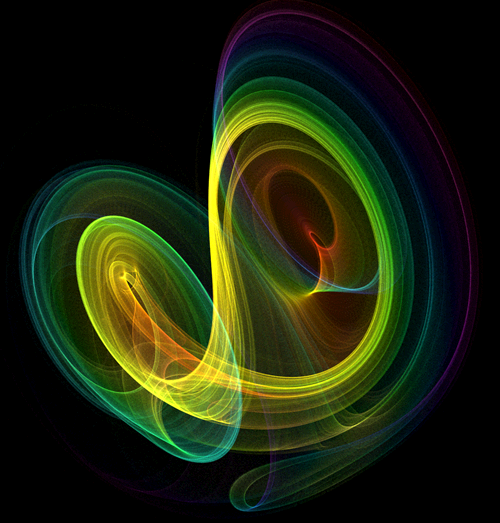
\includegraphics[height=4cm]{lorenz}
 \caption{Illustration de l'attracteur étrange de Lorenz}
 \label{fig:rosen}
\end{figure}

1) Prouvez l'existence de l'attracteur étrange de Lorenz. Détaillez votre réponse.

\end{document}
